\PassOptionsToPackage{table}{xcolor}
\documentclass[sigconf,anonymous,review]{acmart}
\setcopyright{none}
\acmDOI{}
\acmISBN{}
\settopmatter{printacmref=false}
\usepackage{amsmath}
\definecolor{TableInk}{HTML}{284A63}
\definecolor{TableHeader}{HTML}{EAF0F6}
\definecolor{TransferHighlight}{HTML}{E4F1ED}
\definecolor{ConflictHighlight}{HTML}{FFF0DD}
\definecolor{TableStripe}{HTML}{F5F8FA}

\graphicspath{{figures/}}
\begin{document}
\title{Current Figure and Table Reference}
\author{Anonymous Author(s)}
\maketitle
This file collects the current manuscript displays. Recovery is defined as
\begin{equation}
\rho=\frac{\mathrm{acc}(\mathrm{patch})-\mathrm{acc}(\mathrm{receiver})}
{\mathrm{acc}(\mathrm{donor})-\mathrm{acc}(\mathrm{receiver})}.
\label{eq:rho}
\end{equation}
Source-attention dependence is $d(L)=1-q(L)$, the fraction of originally
correct answers lost under cumulative source-attention knockout.
\begin{figure*}[t]
\centering
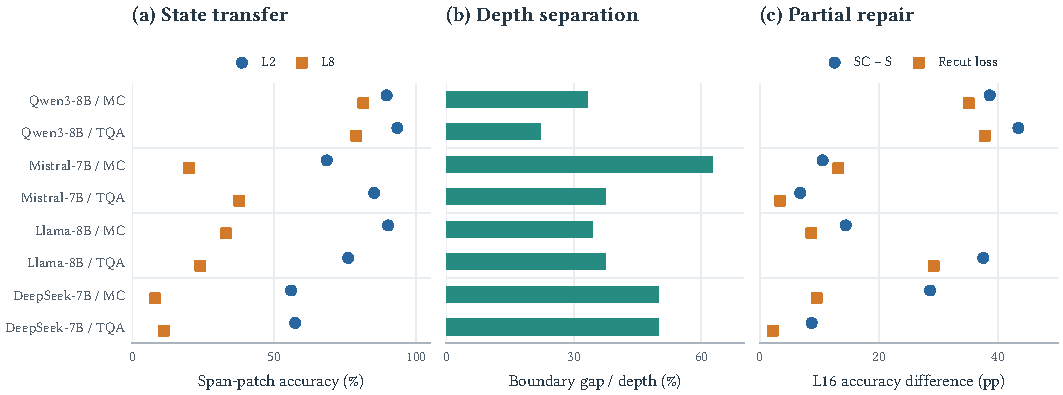
\includegraphics[width=\textwidth]{fig-teaser.pdf}
\caption{Overview of all four main models on both benchmarks (MC: MedCalc;
TQA: TheoremQA). (a) Skill-span replacement accuracy at layers 2 and 8,
with each battery's own baseline-screened population. (b) The gap between
first transfer and dependence boundaries, as a percentage of model depth,
on common eligible items. (c) Fixed-layer-16 joint-repair gain over state
replacement and the loss after a next-layer recut. Panels use separate
protocol-specific populations, not a single item-level trajectory.}
\Description{Eight model--benchmark rows show early versus later transfer, positive normalized boundary gaps, and partial repair followed by recut losses.}
\label{fig:teaser}
\end{figure*}

\clearpage
\begin{figure*}[t]
\centering
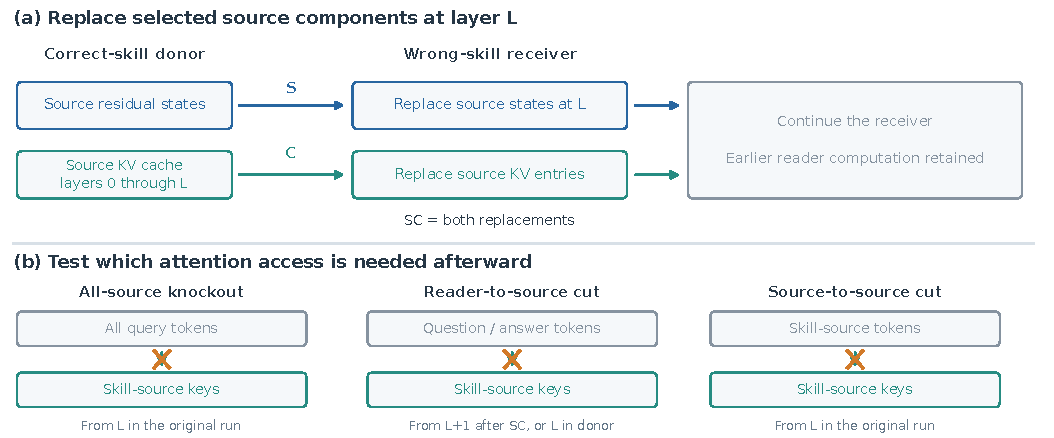
\includegraphics[width=\textwidth]{fig-intervention-design.pdf}
\caption{Intervention design. (a) The correct-skill donor supplies source
residual states ($S$), source-position key/value (KV) entries through layer $L$ ($C$),
or both ($SC$) to the wrong-skill receiver. Earlier reader computation
is retained. (b) Attention cuts distinguish access by reader tokens
from updates within the skill source. After $SC$, the reader cut begins
at $L+1$. In the original correct-skill run, path cuts begin at $L$.
All cuts continue through the remaining prompt processing and decoding.}
\Description{A component-level diagram shows donor source states and caches
replacing selected receiver components while earlier reader computation is
retained. Three attention paths illustrate cumulative knockout, reader cuts
and source-self cuts.}
\label{fig:design}
\end{figure*}

\clearpage
\begin{figure*}[t]
\centering
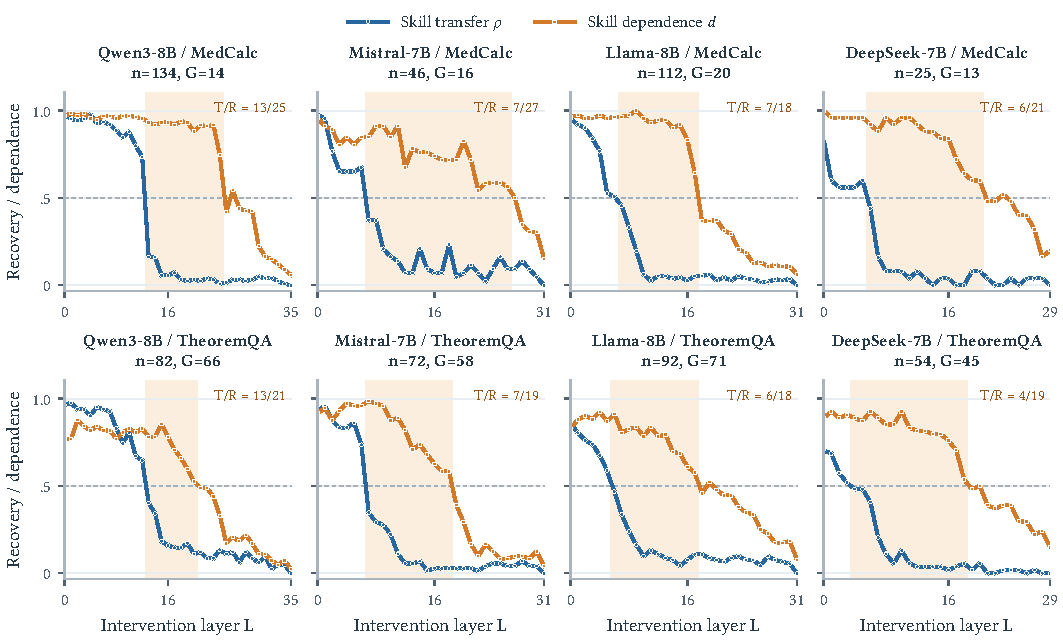
\includegraphics[width=\textwidth]{fig-transfer-reading.pdf}
\caption{Depth profiles for all eight main model--benchmark comparisons. Blue shows
skill-span transfer recovery $\rho(L)$ in a wrong-skill receiver.
Orange shows aggregate skill-attention dependence $d(L)=1-q(L)$: the fraction
of originally correct answers lost after cumulative attention knockout
in the correct-skill execution. Shading spans the first half-effect
boundaries, highlighting weak transfer despite strong dependence; later
recrossings remain visible. Boundary layers are marked above each panel.
Each panel uses common eligible item IDs for both curves, with each run's
own baselines and execution protocol; $G$ denotes skill groups. The
knockout affects both access from post-skill tokens and skill-state updates. Every plotted
layer is measured.}
\Description{Eight line plots show transfer recovery declining before skill-attention dependence subsides on their common eligible populations.}
\label{fig:transferreading}
\end{figure*}

\clearpage
\begin{figure*}[t]
\centering
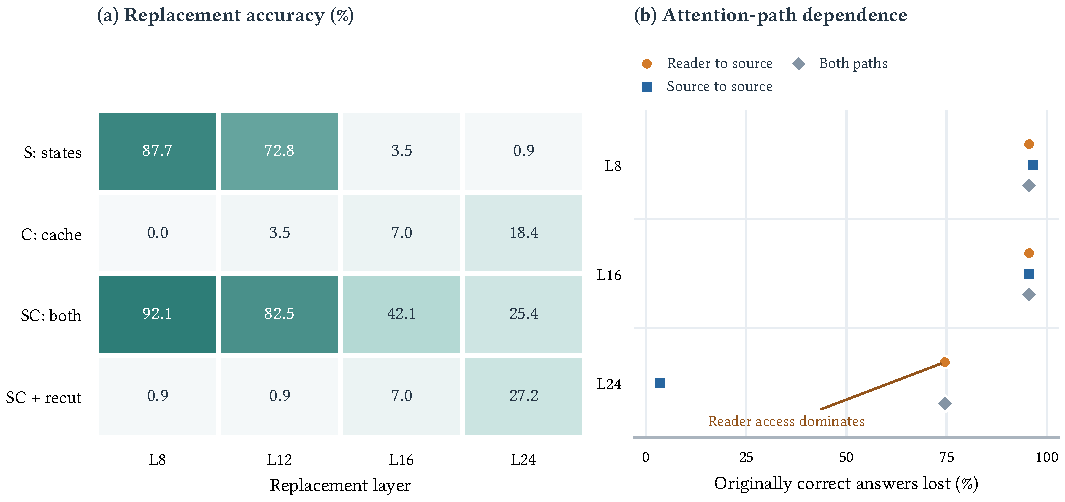
\includegraphics[width=\textwidth]{fig-mechanism-results.pdf}
\caption{Repair and attention-path results for all eight main combinations.
MC denotes MedCalc and TQA denotes TheoremQA. Each row uses its own fresh
split-prefill population; parentheses give questions/skill groups.
(a) Layer-16 accuracy after state ($S$), cache ($C$), joint ($SC$), or joint
replacement followed by a next-layer post-skill-to-skill recut.
(b) At layer 24, the fraction of donor-correct answers lost after cutting
post-skill-to-skill, skill-to-skill, or both paths. Both prefill and decoding
are intervened on. Table~\ref{tab:mechanism-contrasts} gives derived contrasts.}
\Description{Eight rows compare four repair accuracies at layer 16 and three attention-path losses at layer 24 across four models and two benchmarks.}
\label{fig:mechanism}
\end{figure*}

\clearpage
\begin{table*}[t]
\centering
\caption{State-transfer controls for all eight model--benchmark combinations.
Entries are accuracy percentages. $n_2/n_8$ gives the independent layer-2/layer-8
populations; the remaining controls are at layer 8. Other denotes matched-prefix
other-skill content. Qwen3-8B/MedCalc retains its historical layer-8 screen
(124/135 correct donor answers); other batteries require fresh correct donors.
Layer 8 can already lie beyond a model's transfer boundary.}
\label{tab:probe}
\setlength{\tabcolsep}{3pt}
\begin{tabular*}{\textwidth}{@{\extracolsep{\fill}}llrrrrrrrr@{}}
\toprule
Model & Task & $n_2/n_8$ & L2 span & L8 span & Last 1 & Last 16 & Other & Permuted & Noise \\
\midrule
Qwen3-8B & MedCalc & $97/135$ & $89.7$ & $81.5$ & $3.0$ & $5.9$ & $4.4$ & $4.4$ & $2.2$ \\
Qwen3-8B & TheoremQA & $61/57$ & $93.4$ & $78.9$ & $10.5$ & $12.3$ & $14.0$ & $22.8$ & $19.3$ \\
Mistral-7B & MedCalc & $35/35$ & $68.6$ & $20.0$ & $5.7$ & $8.6$ & $2.9$ & $14.3$ & $8.6$ \\
Mistral-7B & TheoremQA & $61/61$ & $85.2$ & $37.7$ & $1.6$ & $6.6$ & $8.2$ & $14.8$ & $4.9$ \\
Llama-3.1-8B & MedCalc & $112/112$ & $90.2$ & $33.0$ & $2.7$ & $2.7$ & $8.0$ & $4.5$ & $4.5$ \\
Llama-3.1-8B & TheoremQA & $92/92$ & $76.1$ & $23.9$ & $12.0$ & $4.3$ & $9.8$ & $14.1$ & $9.8$ \\
DeepSeek-7B & MedCalc & $25/25$ & $56.0$ & $8.0$ & $0.0$ & $4.0$ & $8.0$ & $4.0$ & $4.0$ \\
DeepSeek-7B & TheoremQA & $54/54$ & $57.4$ & $11.1$ & $1.9$ & $11.1$ & $5.6$ & $5.6$ & $0.0$ \\
\bottomrule
\end{tabular*}

\end{table*}

\clearpage
\begin{table}[t]
\centering
\caption{Boundary layers on common eligible items. $T/R$ gives the
first half-effect crossings for transfer ($\rho<0.5$) and source
dependence ($d\le0.5$),
respectively. $\Delta=R-T$ measures their separation in layers. }
\label{tab:paireddepth}
\small
\renewcommand{\arraystretch}{1.18}
\setlength{\tabcolsep}{4pt}
\begin{tabular}{@{}llrcc@{}}
\toprule
\textbf{Task} & \textbf{Model} & $n$ & $T/R$ & $\Delta$ \\
\midrule
MedCalc & Qwen3-8B & $134$ & $13/25$ & $12$ \\
MedCalc & Qwen3-0.6B & $90$ & $11/22$ & $11$ \\
MedCalc & Mistral-7B & $46$ & $7/27$ & $20$ \\
MedCalc & Llama-8B & $112$ & $7/18$ & $11$ \\
MedCalc & DeepSeek-7B & $25$ & $6/21$ & $15$ \\
\midrule
TheoremQA & Llama-8B & $92$ & $6/18$ & $12$ \\
TheoremQA & DeepSeek-7B & $54$ & $4/19$ & $15$ \\
\bottomrule
\end{tabular}

\end{table}

\clearpage
\begin{table*}[t]
\centering
\caption{Mechanism contrasts for all eight main combinations, in percentage points.
$n/G$ gives each row's questions/skills. With accuracy $a_X$, interaction is
$a_{SC}-a_S-a_C+a_R$; recut loss is $a_{SC}-a_{SC+\mathrm{recut}}$.
The L24 path gap is skill-to-skill-cut accuracy minus post-skill-to-skill-cut
accuracy, equivalently the excess loss from cutting post-skill access.}
\label{tab:mechanism-contrasts}
\setlength{\tabcolsep}{3pt}
\begin{tabular*}{\textwidth}{@{\extracolsep{\fill}}llrrrrr@{}}
\toprule
Model & Task & $n/G$ & L16: $SC-S$ & L16: interaction & L16: recut loss & L24: path gap \\
\midrule
Qwen3-8B & MedCalc & $114/14$ & $+38.6$ & $+31.6$ & $+35.1$ & $+71.1$ \\
Qwen3-8B & TheoremQA & $53/43$ & $+43.4$ & $+28.3$ & $+37.7$ & $+18.9$ \\
Mistral-7B & MedCalc & $38/15$ & $+10.5$ & $-7.9$ & $+13.2$ & $+23.7$ \\
Mistral-7B & TheoremQA & $59/49$ & $+6.8$ & $+1.7$ & $+3.4$ & $+6.8$ \\
Llama-3.1-8B & MedCalc & $104/20$ & $+14.4$ & $+8.7$ & $+8.7$ & $+13.5$ \\
Llama-3.1-8B & TheoremQA & $72/56$ & $+37.5$ & $+25.0$ & $+29.2$ & $+9.7$ \\
DeepSeek-7B & MedCalc & $21/10$ & $+28.6$ & $+9.5$ & $+9.5$ & $+42.9$ \\
DeepSeek-7B & TheoremQA & $46/40$ & $+8.7$ & $+2.2$ & $+2.2$ & $+17.4$ \\
\bottomrule
\end{tabular*}

\end{table*}

\clearpage
\begin{table*}[tbp]
\caption{Cross-question transfer and repeated-write controls for all eight main
combinations. Current/Other compare skill-after-question donors at layer 8;
$n_{\rm cross}/n_{\rm win}$ gives independent populations. W indicates the inclusive
write window. Acc. is raw accuracy; the historical Qwen3-8B/MedCalc row uses
normalized recovery $\rho$ with its own donor/receiver baselines.
Rows with different units are not accuracy rankings. Windows ending at the last
layer depend on model depth.}
\label{tab:fullscale}
\centering
\setlength{\tabcolsep}{2pt}
\begin{tabular*}{\textwidth}{@{\extracolsep{\fill}}llrlrrrrrr@{}}
\toprule
Model & Task & $n_{\rm cross}/n_{\rm win}$ & Unit & Current & Other & W8--11 & W12--15 & W14--19 & W16--end \\
\midrule
Qwen3-8B & MedCalc & $151/135$ & $\rho$ & $1.02$ & $0.98$ & $0.89$ & $0.74$ & $0.16$ & $0.06$ \\
Qwen3-8B & TheoremQA & $8/61$ & Acc. & $0.88$ & $0.88$ & $0.79$ & $0.61$ & $0.38$ & $0.25$ \\
Mistral-7B & MedCalc & $10/35$ & Acc. & $0.40$ & $0.10$ & $0.20$ & $0.14$ & $0.09$ & $0.09$ \\
Mistral-7B & TheoremQA & $7/61$ & Acc. & $0.86$ & $0.57$ & $0.38$ & $0.07$ & $0.07$ & $0.07$ \\
Llama-3.1-8B & MedCalc & $92/112$ & Acc. & $0.50$ & $0.39$ & $0.33$ & $0.05$ & $0.04$ & $0.03$ \\
Llama-3.1-8B & TheoremQA & $46/92$ & Acc. & $0.41$ & $0.33$ & $0.24$ & $0.11$ & $0.08$ & $0.08$ \\
DeepSeek-7B & MedCalc & $25/25$ & Acc. & $0.96$ & $0.92$ & $0.08$ & $0.08$ & $0.00$ & $0.04$ \\
DeepSeek-7B & TheoremQA & $23/54$ & Acc. & $0.39$ & $0.35$ & $0.11$ & $0.04$ & $0.04$ & $0.02$ \\
\bottomrule
\end{tabular*}

\end{table*}

\clearpage
\end{document}
